\documentclass[12pt]{article}
\usepackage[utf8]{inputenc}
\usepackage[margin=0.7in]{geometry}
\usepackage{titlesec}
\usepackage{graphicx}
\usepackage[english]{babel}
\usepackage{fancyhdr}
\usepackage{blindtext}
\usepackage{textcomp}
\pagestyle{fancy}
\fancyhf{}
\rhead{Sam Robbins 13SE}
\lhead{A Level Physics - Turning Points}
\begin{document}
\begin{center}
\underline{\huge The Significance of Young’s double slit experiment}
\end{center}
\section{Explanation for fringes}
Young discovered that the creation of an interference pattern required two light sources that had a constant phase difference and so had to be created from the same original source. Young had discovered how to create coherent sources of light.\\
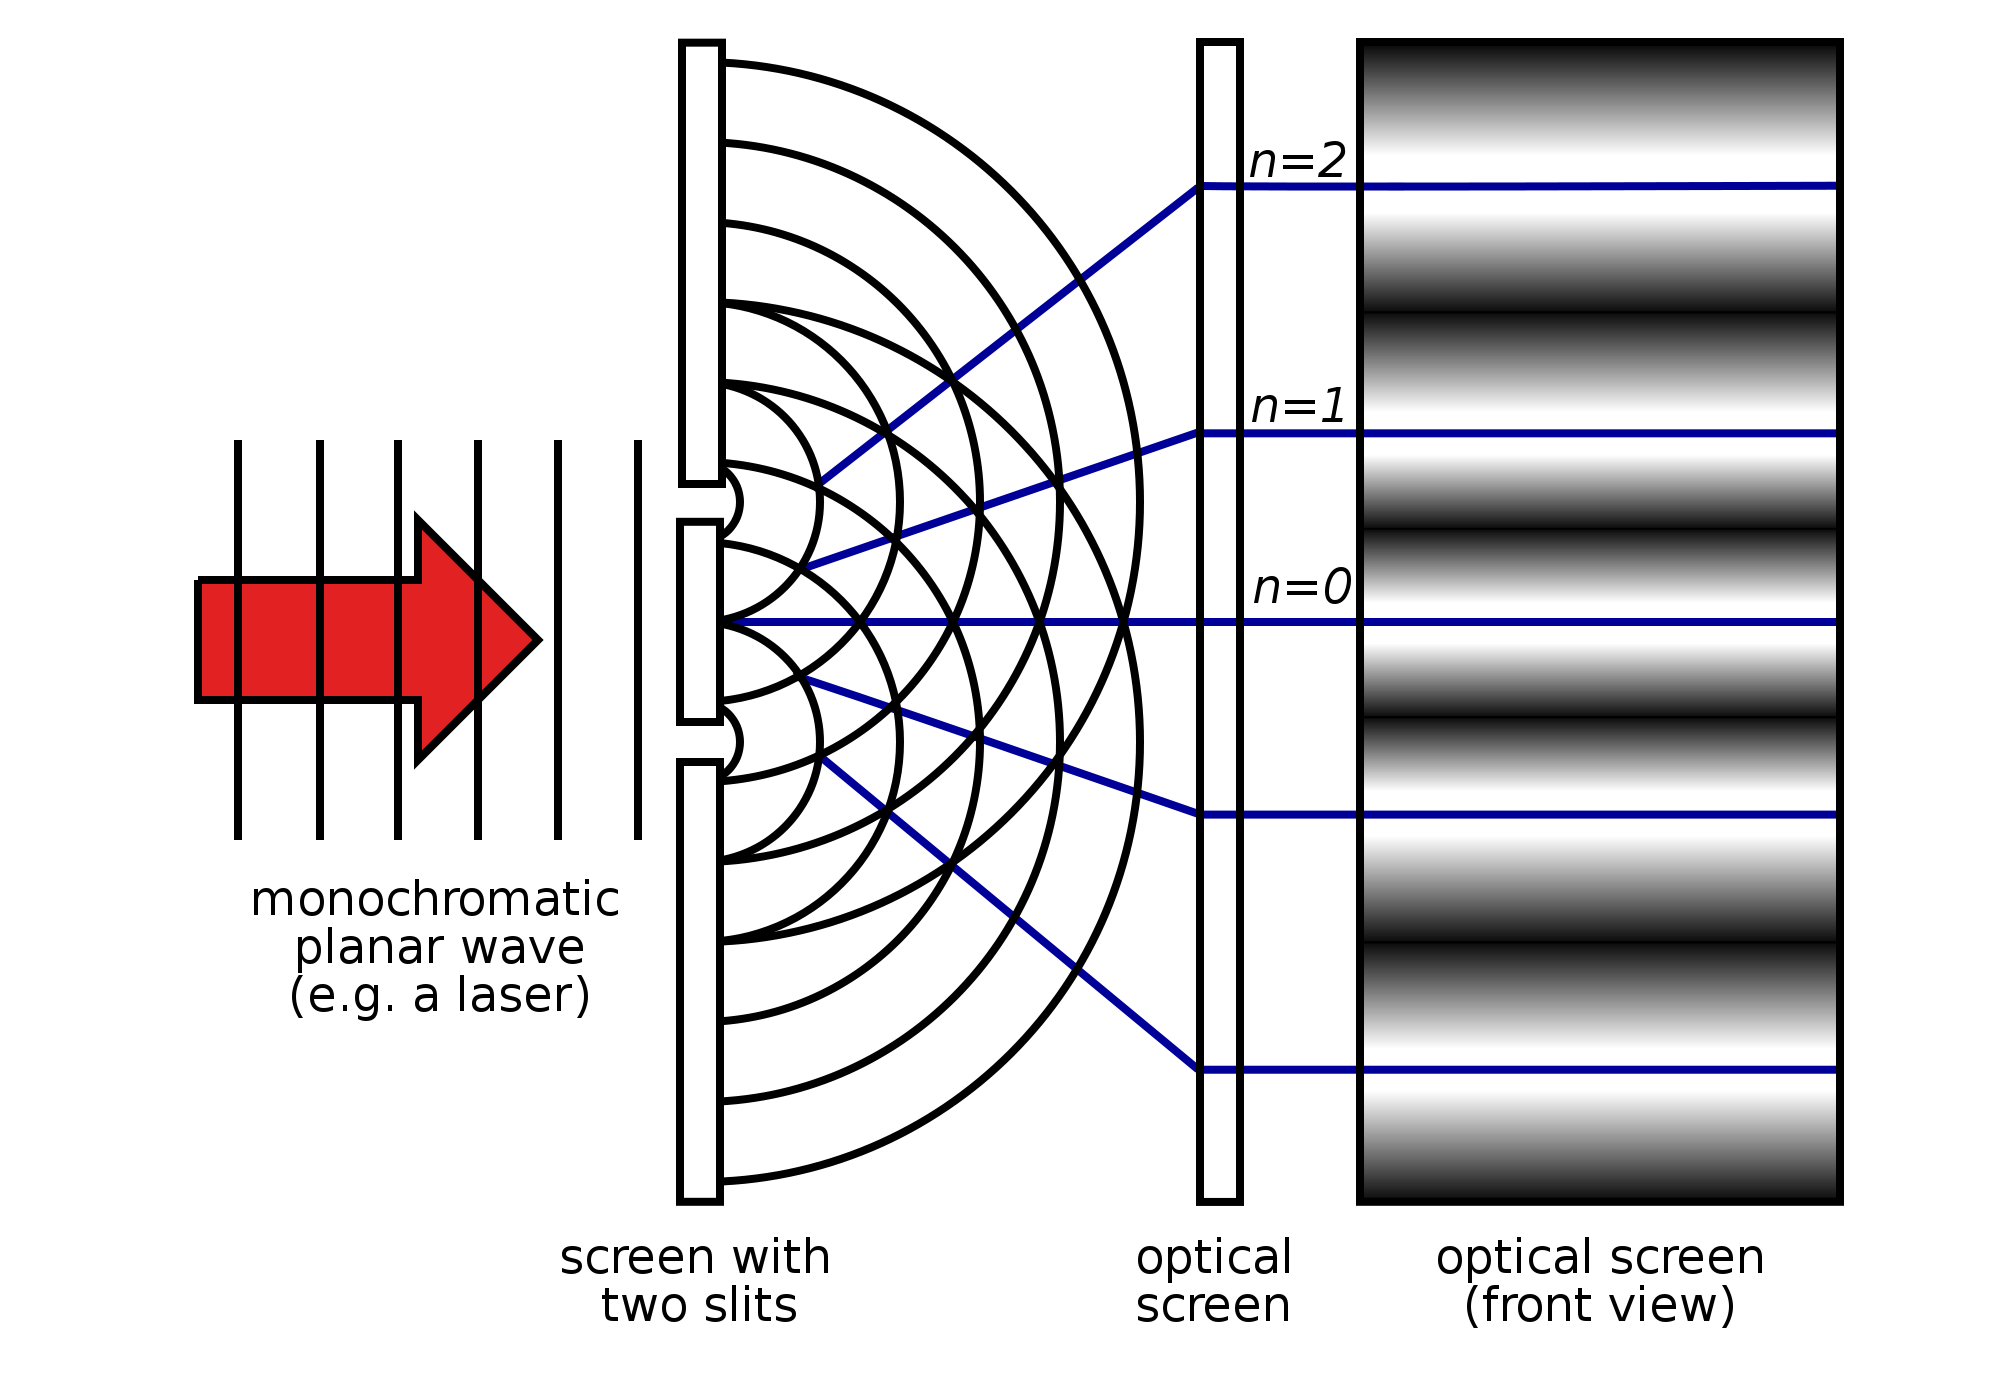
\includegraphics[width=8cm]{double_slit.png}\\
As interference is a wave property, this disproved Newton's Corpuscular Theory and Proved Huygens' Wave front theory.
\section{Delayed acceptance of Huygen's  Wave front theory}
Despite Young's conclusive evidence against Newton's Corpuscular Theory, there was still reluctance to drop the theory.\\
The theory wasn't dropped until Fizeau measured the speed of light in water and air, and calculated that the speed of light in water is slower than that in air, finally disproving Newton's corpuscular theory.
\end{document}